\documentclass[conference]{IEEEtran}
\usepackage{graphicx}
\usepackage{amsmath}

\graphicspath{{./gambar/}}

\title{Analisis kekuatan Sinyal Menggunakan inSSIDer}

\author{Kevin Antony K\IEEEauthorrefmark{1}, Maranti Nainggolan\IEEEauthorrefmark{2}\\
\textit{Fakultas Teknologi Informasi}\\
\textit{Teknik Komputer}\\
\textit{Institut Teknologi Batam}\\
Batam, Indonesia\\
Email: \{\IEEEauthorrefmark{1}1922003, \IEEEauthorrefmark{2}1922023\}@student.iteba.ac.id}

\begin{document}

\maketitle

\begin{abstract}
    
Kemajuan teknologi informasi pada saat ini
terus berkembang seiring dengan kebutuhan manusia yang
menginginkan kemudahan, kecepatan, dan keakuratan dalam
memperoleh informasi. Oleh karena itu kemajuan teknologi
informasi di bidang transmisi pada saat ini yang berkembang
selain fiber optic ialah penggunaan perangkat wireless. Perangkat
wireless ini memungkinkan adanya hubungan para pengguna
informasi dalam melakukan aktivitasnya
\end{abstract}

\begin{IEEEkeywords}
Access Point, InSSIDer, SSID, Wi-Fi.
\end{IEEEkeywords}

\section{Introduction}
Teknologi Wifi atau yang dikenal dengan wireless LAN(WLAN) telah banyak diimplemantasikan 
oleh masyarakat baik didalam maupun diluar negeri.Selain untuk aplikasi privat,WLAN 
juga banyak digunakan untuk aplikasi public(hospot).\

\vspace{0.2cm}

WLAN merupakan jaringan yang tidak tampak karena
merupakan gelombang radio. Terutama bila frekuensinya terlalu
berdekatan, atau hilang oleh daya gelombang radio yang
lebih besar sehingga jaringan yang kita buat menjadi tidak
efisien. Untuk itu diperlukan suatu software yang dapat digunakan
untuk mencari informasi jaringan WLAN pada suatu
area lebih spesifik dari scan biasa. Salah satu software yang
dapat digunakan adalah inSSIDer.\

\vspace{0.2cm}

InSSIDer merupakan software Wi-Fi scanner yang dapat
mengidentifikasi SSID, RSSI (Received Signal Strength Indicator),
security, dan pengaturan yang ada pada AP. Software
ini dikembangkan oleh MetaGeek, LLC dan lain lain.


Kemajuan Teknologi Informasi pada saat ini juga dapat juga dapat


\section{Related Work}

\section{Scenario}

\begin{figure}[htbp]
    \input{gambar/topologi.pdf_tex}
\end{figure}

\section{Hasil dan Pembahasan}
\vspace{0.2cm}

Pada tugas kali ini akan dilakukan pengambilan data.
\begin{enumerate}
    \item Pengambilan data dengan jarak 15 meter dari rumah

    \begin{figure}
        \centering
        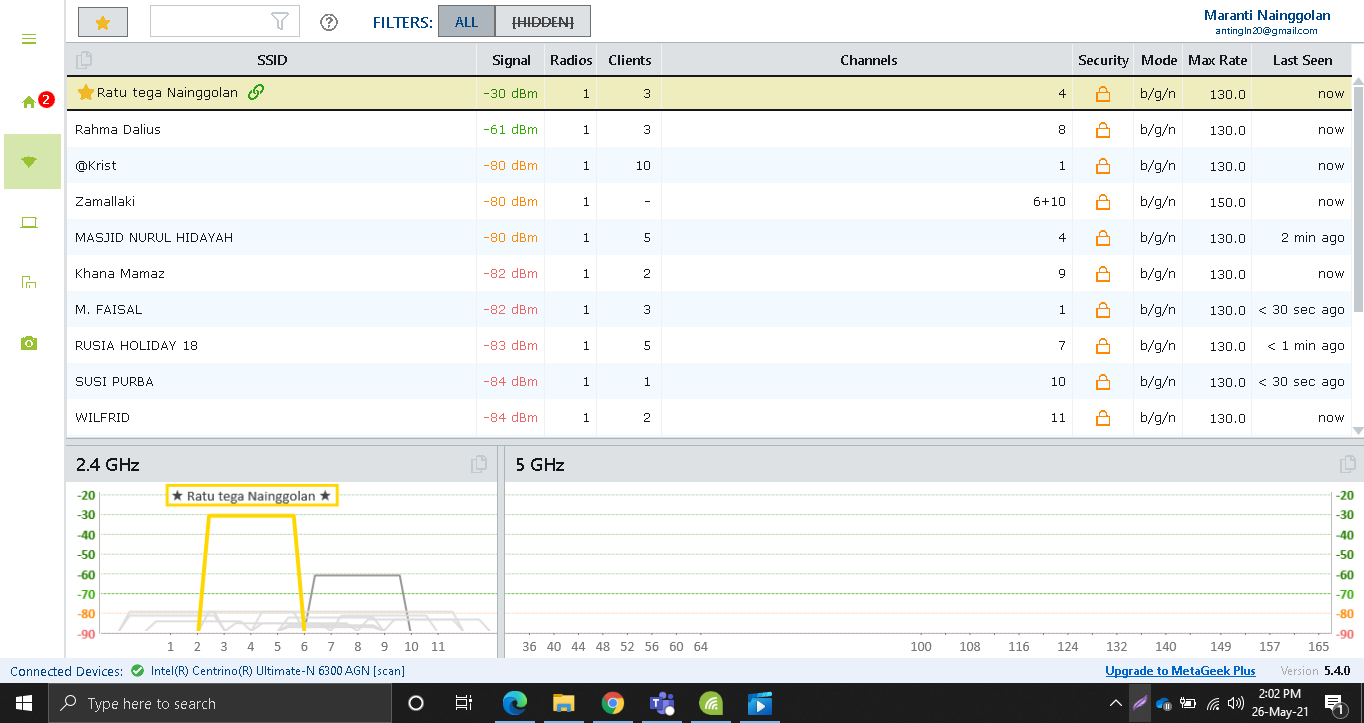
\includegraphics[width=0.4\textwidth]{8.png}
        \caption{Tampilan inSSIDer dalam Rumah}
    \end{figure}

    \begin{figure}
        \centering
        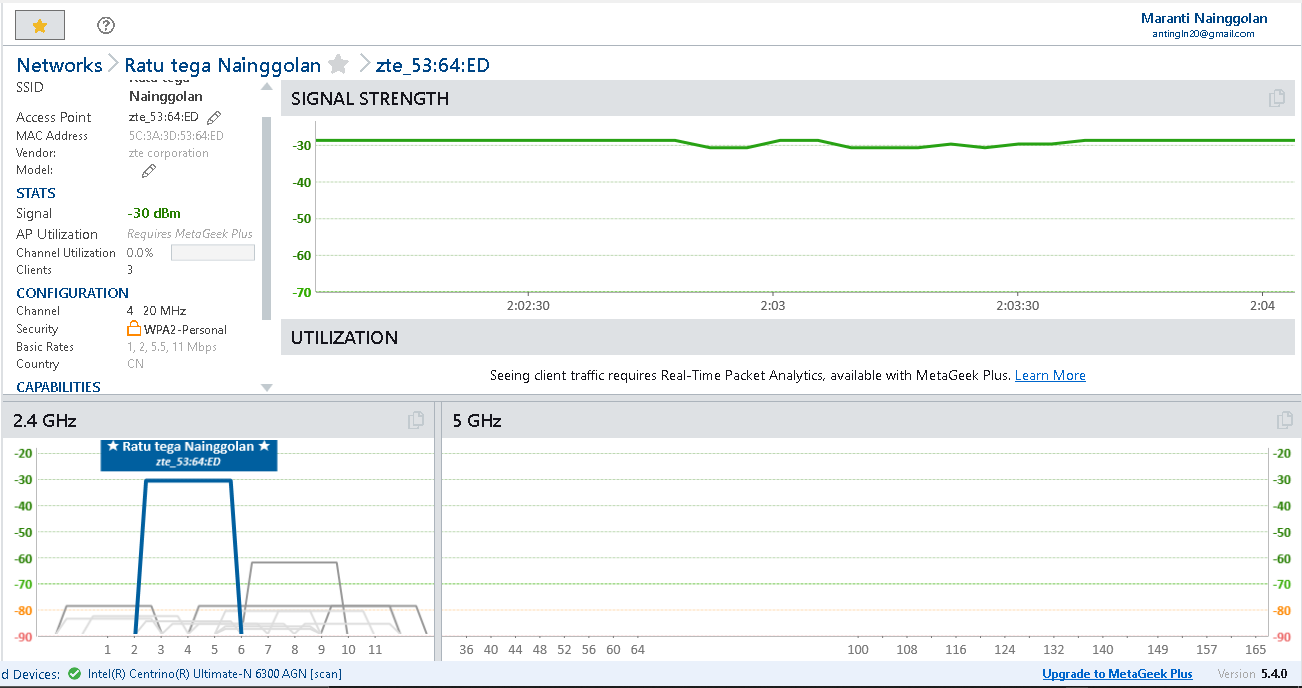
\includegraphics[width=0.4\textwidth]{9.png}
        \caption{Tampilan inSSIDer dalam rumah}
    \end{figure}

\vspace{0.2cm}

Dari AP yang sinyalnya diterima dan tekdeteksi pada inSSIDer terlihat bahwa AP dengan SSID "Ratu tega nainggolan" memiliki 
RSSI (Received Signal Strenght Indicator) yaitu -30 dBm. Seting kanal yang digunakan
adalah kanal 1 dan bekerja pada frekuensi 2,4 GHz. Menggunakan model WPA-2 personal
security dan memiliki channel 4.
\end{enumerate}





\begin{equation}
    Rerata RSSI = \frac{Total Jumlah Nilai RSSI}{Jumlah Koordinat receiver}
    \label{rerata_rssi}
\end{equation}

berdasarkan persamaan~\ref{rerata_rssi}

\section{Kesimpulan}

\bibliographystyle{IEEtran}
\bibliography{referensi.bib}

\end{document}